\documentclass{article}
\usepackage{graphicx} % Required for inserting images
\usepackage{amsmath}
\usepackage[russian]{babel}
\usepackage{float}


\renewcommand{\thesection}{\arabic{section}.}

\title{Методы оптимизации, Лабораторная работа №2}
\author{Кирилл Кадомцев и Андрей Крюков}
\date{Май 2025}

\begin{document}
\maketitle
\tableofcontents

\section{Описание методов}
Был реализован метод Ньютона и метод Ньютона с выбором шага.

Для удобства и расширяемости, методы реализовывались так, чтоб можно было в дальнейшем использовать их для любых размерностей (исходя из предположения, что это может стать объектом исследования в дальнейших лабораторных работах). Для стратегий был создан специальный интерфейс с методом \textit{step}, позволяющий в дальнейшем расширить список реализованных методов.


\section{Тестирование}
Для тестирования были выбраны несколько функций с различными точками минимума. Также, была использованна функция Химмельблау, поскольку она мультимодальная.
\begin{enumerate}
  \item \textbf{Параболоид}
  \begin{itemize}
    \item \( f(x, y) = x^2 + y^2 \)
    \item \( \nabla f(x, y) = \begin{pmatrix} 2x \\ 2y \end{pmatrix} \)
  \end{itemize}

  \item \textbf{Эллипс}
  \begin{itemize}
    \item \( f(x, y) = 4x + y \)
    \item \( \nabla f(x, y) = \begin{pmatrix} 8x \\ 2y \end{pmatrix} \)
  \end{itemize}

  \item \textbf{Функция Розенброка}
  \begin{itemize}
    \item \( f(x, y) = (1 - x)^2 + 100(y - x^2)^2 \)
    \item \( \nabla f(x, y) = \begin{pmatrix}
      -2(1 - x) - 400x(y - x^2) \\
      200(y - x^2)
    \end{pmatrix} \)
  \end{itemize}

  \item \textbf{Квадратичная форма (3, -2)}
  \begin{itemize}
    \item \( f(x, y) = (x - 3)^2 + (y + 2)^2 \)
    \item \( \nabla f(x, y) = \begin{pmatrix}
      2(x - 3) \\
      2(y + 2)
    \end{pmatrix} \)
  \end{itemize}

  \item \textbf{Квадратичная форма (2, -1)}
  \begin{itemize}
    \item \( f(x, y) = x + y \)
    \item \( \nabla f(x, y) = \begin{pmatrix}
      10(x - 2) \\
      6(y + 1)
    \end{pmatrix} \)
  \end{itemize}

  \item \textbf{Функция Химмельблау}
  \begin{itemize}
    \item \( f(x, y) = (x^2 + y - 11)^2 + (x + y^2 - 7)^2 \)
    \item \( \nabla f(x, y) = \begin{pmatrix}
      4x(x^2 + y - 11) + 2(x + y^2 - 7) \\
      2(x^2 + y - 11) + 4y(x + y^2 - 7)
    \end{pmatrix} \)
  \end{itemize}
\end{enumerate}

Ниже приведены результаты оптимизации в зависимости от стратегии выбора шага. В данном случае \textit{(nan, nan)} является результатом переполнения, то есть провалом поиска минимума.


\begin{table}[H]
\centering
%\small
\begin{tabular}{|l|c|c|c|}
\hline
\textbf{Функция} & \textbf{Корни} & \textbf{Backtracking} & \textbf{Пост. шаг} \\
\hline
paraboloid & \( (0,\ 0) \) & \( (0,\ 0) \) & \( (0,\ 0) \) \\
\hline
ellipse & \( (0,\ 0) \) & \( (0,\ 0) \) & \( (0,\ 0) \) \\
\hline
rosenbrock & \( (1,\ 1) \) & \( (0.99995,\ 0.99990) \) & \( (1.0000,\ 1.0000) \) \\
\hline
min3m2 & \( (3,\ -2) \) & \( (3.0000,\ -2.0000) \) & \( (3.0000,\ -2.0000) \) \\
\hline
min2m1 & \( (2,\ -1) \) & \( (0.0000,\ 0.0000) \) & \( (2.0000,\ -1.0000) \) \\
\hline
himmelblau & 
\(
\begin{array}{l}
(3.0,\ 2.0),\ (-2.8051,\ 3.1313), \\
(-3.7793,\ -3.2832),\ (3.5844,\ -1.8481)
\end{array}
\) 
& \( (0.0000,\ 0.0000) \) & \( (-0.3423,\ 0.2500) \) \\
\hline
\end{tabular}
\caption{Сравнение приближений к корням \( f(x, y) = 0 \) при использовании метода Ньютона с разными стратегиями шага}
\end{table}

\section{Графики}
Не будем приводить все графики ввиду избыточности. Графики для эллипса демонстрируют, что точка минимума $(0, 0)$ находится за 1 итерацию. Графики для функции Химмельблау показывают несовершенство постоянного и кусочно-постоянного методов для мультимодальной функции. Для квадратичной функции графики приведены для демонстрации работы корректности работы в случае, если минимум отличен от нуля.
\begin{figure}[H]
    \centering
    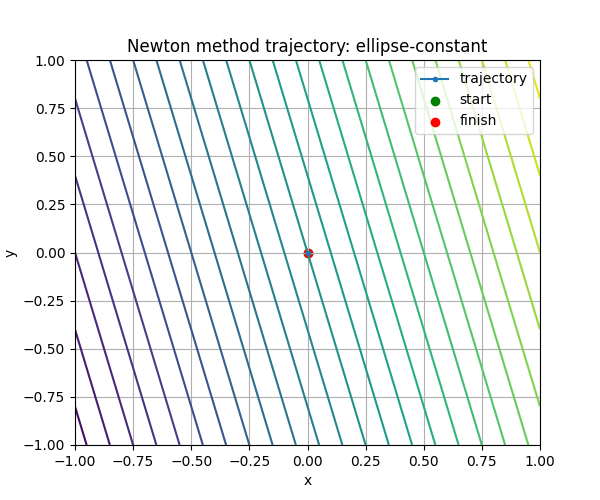
\includegraphics[width=1\linewidth]{ellipse-constant.png}
    \label{fig:enter-label}
\end{figure}
\begin{figure}[H]
    \centering
    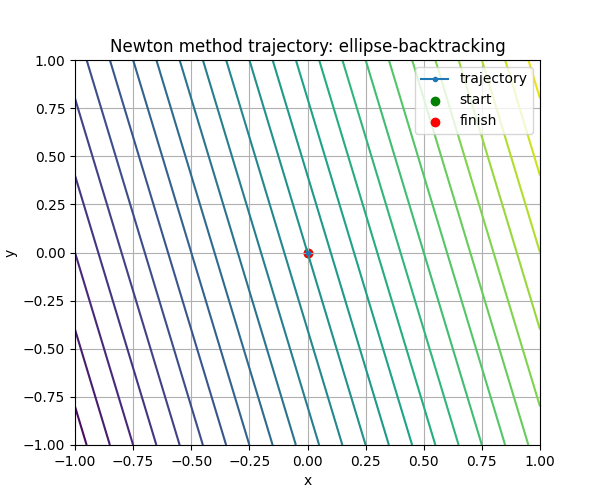
\includegraphics[width=1\linewidth]{ellipse-backtracking.png}
    \label{fig:enter-label}
\end{figure}
\begin{figure}[H]
    \centering
    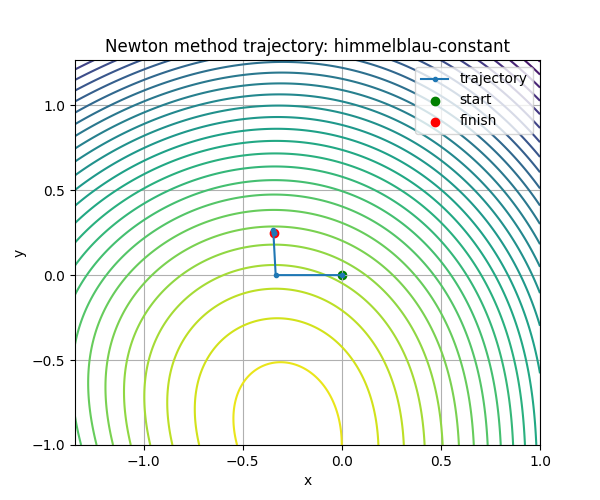
\includegraphics[width=1\linewidth]{himmelblau-constant.png}
    \label{fig:enter-label}
\end{figure}
\begin{figure}[H]
    \centering
    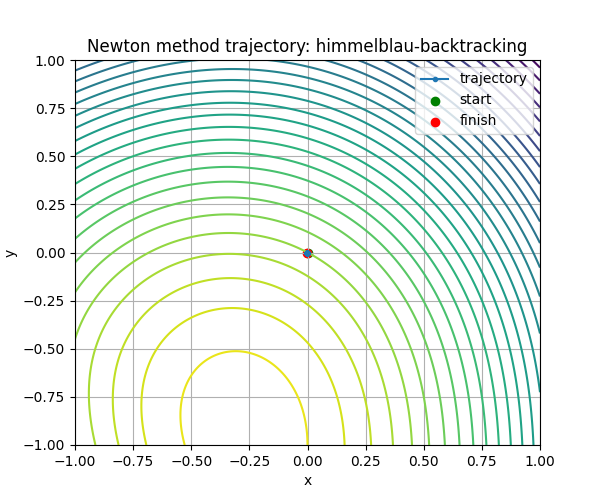
\includegraphics[width=1\linewidth]{himmelblau-backtracking.png}
    \label{fig:enter-label}
\end{figure}
\begin{figure}
    \centering
    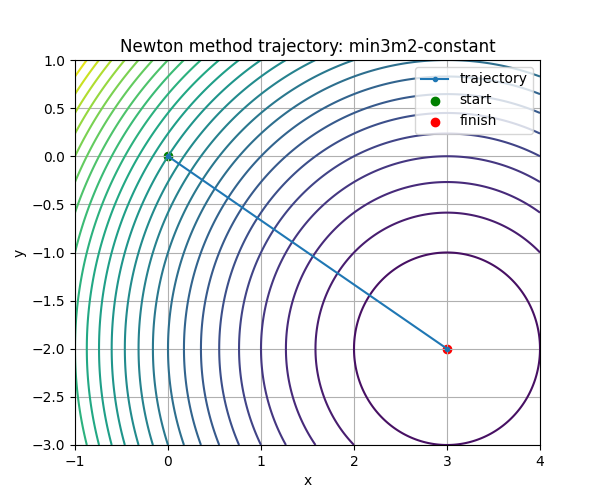
\includegraphics[width=1\linewidth]{min3m2-constant.png}
    \label{fig:enter-label}
\end{figure}
\begin{figure}
    \centering
    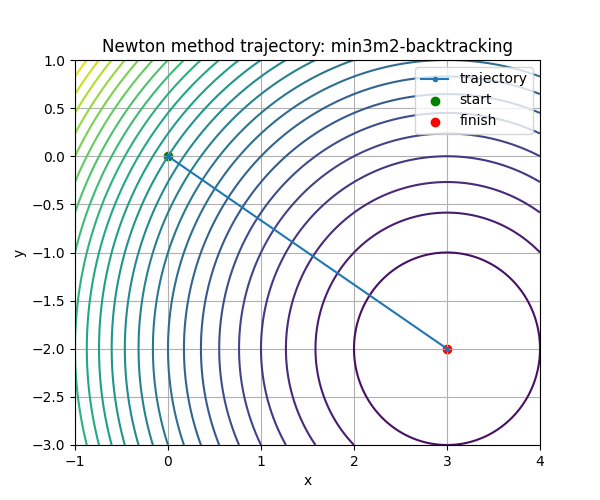
\includegraphics[width=1\linewidth]{min3m2-backtracking.png}
    \label{fig:enter-label}
\end{figure}
\end{document}